\chapter{Introduction}
\pagenumbering{arabic}\hspace{3mm}

Ever since machine learning has been introduced into the field of computer science, it has been spearheading breakthroughs in a number of fields. It has taken the world by storm and now, many fields will simply cease to function without these techniques. Deep learning is one sub-field of machine learning which is deeply rooted in todays society. Deep learning is now part of common man's everyday life and it will remain so for the forseeable future.

As data collection and storage becomes more prominent, machine and deep learning has continued to dominate the data space, provide insights into complex data which is simply not possible with other mathematical methods. Deep learning is one of the most rapidly expanding machine learning technologies, relying on multi-layered artificial neural networks (ANNs) implemented in digital electronics to handle big data sets, integrating and analysing massive volumes of information quickly without the need for explicit instructions. These ANNs have been modified and augmented in many ways, leading many domain specific techniques, most notable one being Convolutional Neural Networks (CNNs) which is primarily used in image analysis.

\section{Artifical Neural Networks}

Artificial neural networks refers to those algorithms which are inspired by the biological neural networks that constitute animal brains. Such systems learn to perform tasks by considering examples, generally without being programmed with any task-specific rules. For example, in image recognition, they might learn to identify images that contain cats by analyzing example images that have been manually labeled as "cat" or "no cat" and using the results to identify cats in other images. They have found most use in applications difficult to express with a traditional computer algorithm using rule-based programming.

Traditionally ANNs have been described as a black box of sorts. It has a number of input variables and output variables using simple arithmetic connections, gives output from the input.

\begin{figure}
	\centering
	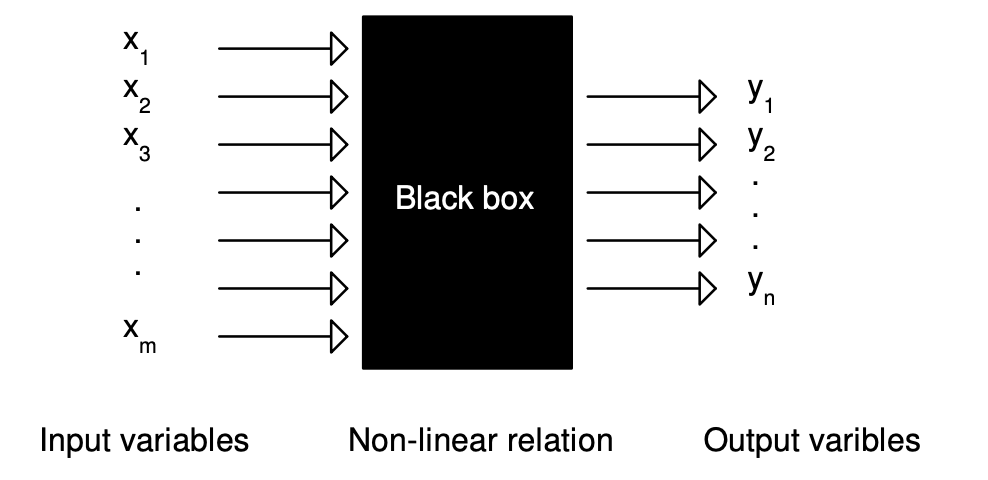
\includegraphics[width=0.5\textwidth]{images/ann.png}
	\caption{Blackbox representation of a ANN}
	\label{fig:neuron}
\end{figure}

ANNs Traditionally tend to excel where the relations between inputs and outputs are non-linear. It is practically better and more efficient at classifying or identifying non-linear relationships rather that linear ones, where it might perform worse than a more statistical approach.

Nowadays, the most common type of ANN is the feedforward neural network, which consists of a group of neurons (called a layer) that transfer data to another group of neurons in a feedforward manner. The first layer is called the input layer, and the last layer is called the output layer. The layers in between are called hidden layers. The input data travels through the layers in a feedforward manner, and the output is the result of the last layer. The output is then compared to the expected output, and the error is calculated. The error is then backpropagated through the network, and the weights are adjusted accordingly. This process is repeated until the error is below a certain threshold.

\begin{figure}[h]
	\centering
	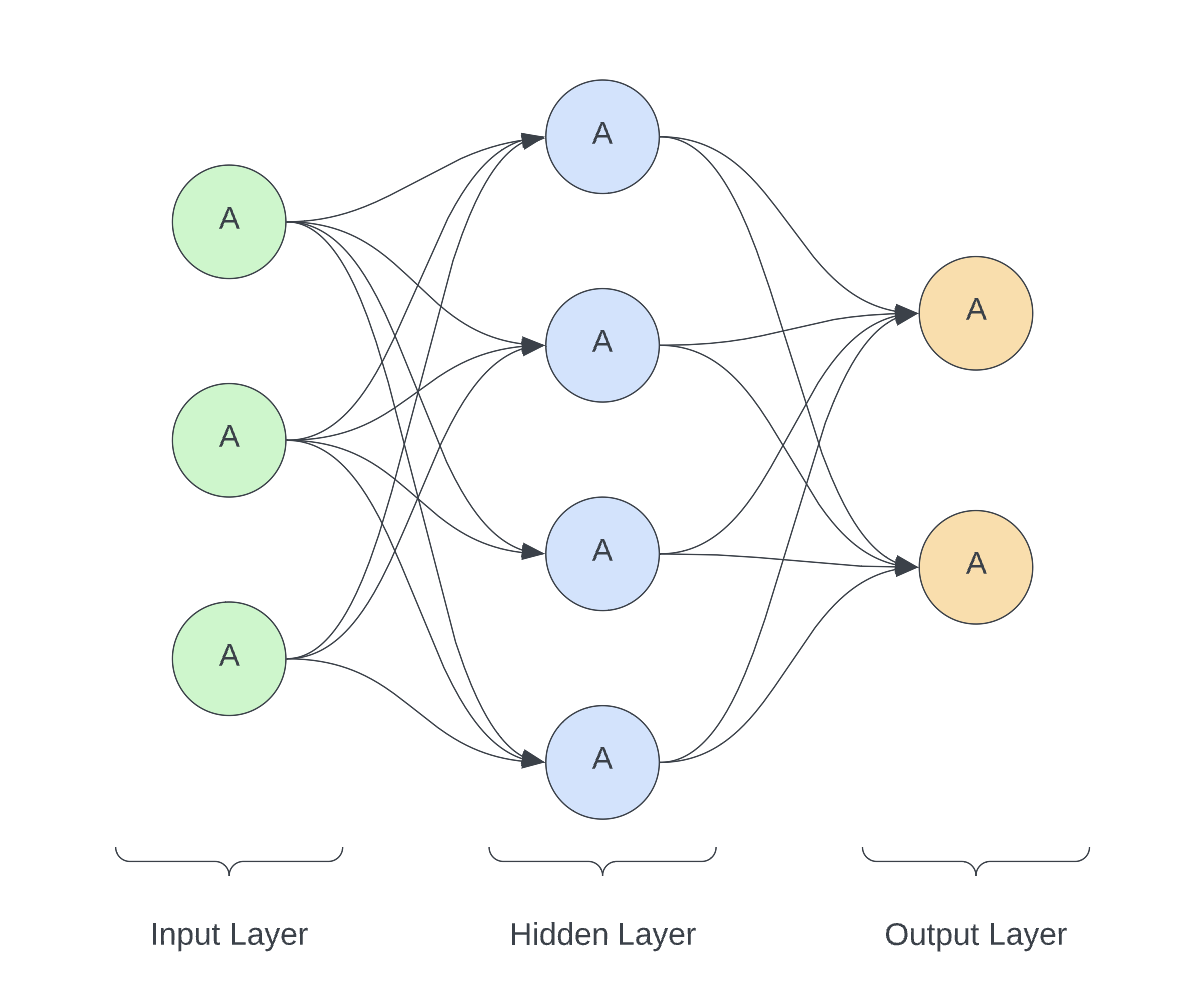
\includegraphics[width=0.7\textwidth]{images/feedforwardANN.png}
	\caption{Feedforward ANN}
\end{figure}

\section{Convolutional Neural Networks}

Convolutional Neural Networks (CNNs) are a class of deep neural networks, most commonly applied to analyzing visual imagery. They are also known as shift invariant or space invariant artificial neural networks (SIANN), based on their shared-weights architecture and translation invariance characteristics. They have applications in image and video recognition, recommender systems, image classification, medical image analysis, natural language processing, brain-computer interfaces, and financial time series.

CNNs usually apply convolution operation over the image (hence the name) by using a filter, called the kernel. This produces a smaller image but where features can be extracted easily. Diiferent filters are applied to the same image in the form of multiple channels resulting in diverging features in each channel which can be detected. This is called feature mapping. The feature maps are then flattened and fed into a fully connected ANN which gives the final output. The application of kernel is illustrated in figure \ref{cnn}.
\\
\begin{figure}[h]
	\centering
	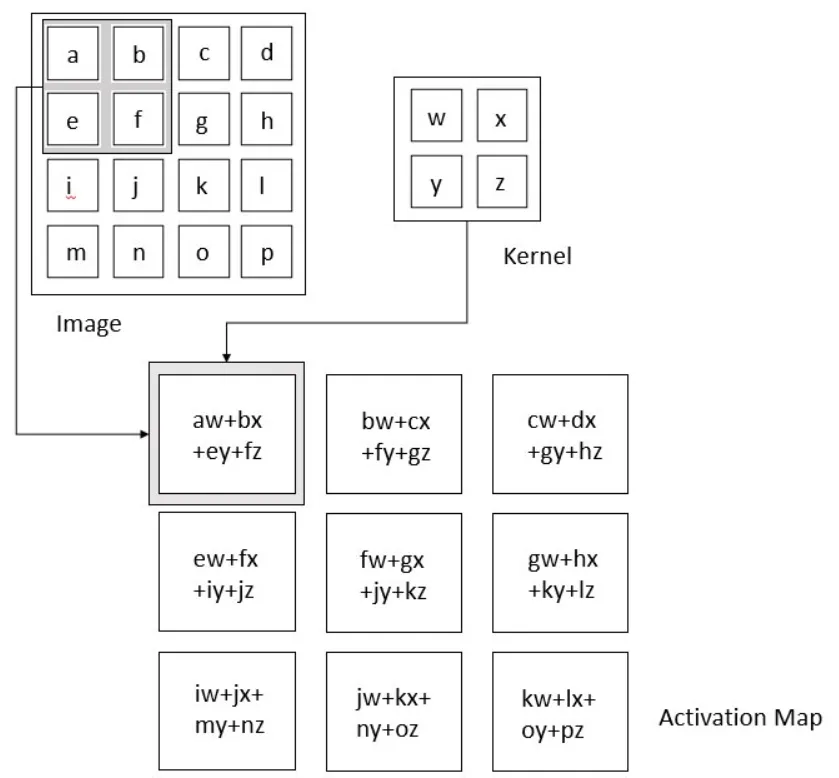
\includegraphics[width=0.8\textwidth]{images/cnn.png}
	\caption{Working of kernel and convolution in CNNs \cite{Goodfellow-et-al-2016}}
	\label{cnn}
\end{figure}

\section{Conventional Implementation of Neural Networks}

Neural networks, for the most part, have been software based. The algorithms are implemented in code and is executed in high-power GPUs for fast parallel computations. This form is extremely flexible and can be used for a variety of applications. The model can be changed as and when the need arises and is reletively commitment-less. The hardware itself is also largely independent of the software and changed/replaced whenever deemed necessary.

There has been a recent growth in certain of Application Specific Integrated Circuits (ASICs) specifically for neural networks, some notable examples being from popular manufactors like NVIDIA \cite{NVIDIAT4Tensor} and Apple. These chips are designed to perform neural network computations and are extremely fast and efficient. They are also extremely expensive and are not easily available.

Even with the advent of ASICs in Machine learning space, the field still suffers from the fact that the hardware is not really coupled with the software. By increasing the specificity of the hardware, the efficiency of the system can be increased by a large margin.

\section{Disadvantages of Conventional Implementation}

The conventional implementation of neural networks has a number of disadvantages. The most prominent one being the fact that the hardware is not really coupled with the software. The hardware is not really designed to perform neural network computations and is not really efficient at it. Large amounts of power are required to train models for prolonged amounts of time. This leads to a lot of inefficiencies in the system.

\section{Photonic Neuron}

As discussed, the conventional implementation of neural networks has a number of disadvantages. The hardware is not really designed to perform neural network computations and is not really efficient at it. This sparks the question "What can be a proper hardware implementation of neuron, the basic structure of a neural network, that can be used to perform neural network computations efficiently?". The answer to this question that this thesis proposes is the Photonic Neuron.

The photonic neuron exploits the fact that multiplication can be done essentially for free in the photonics domain through the use fo hardware like Mach-Zehnder Interferometers or Micro-Ring Resonators. Photonics is known to be inherently very fast since most of the operations are done in speeds close to the speed of light. This makes it a very good candidate for the speed up of existing hardware implementation.

Many prospective applications become blaringly obvious when we consider the speeds that photonics really has to offer. When we also consider the power efficiency of such a implementation, we can see the possibilities. Easily identifiable applications include on-device deployments of trained models for applications like self-driving cars, drones, etc. These require highly power efficient and latentcy-less neural network implementation which photonics can offer.

\section{Diiferent Architectures of Photonic Neurons}

There are a number of different architectures of photonic neurons that have been proposed. Some of them are discussed below.

One possible implementation is cascading a number of Mach-Zehnder Interferometers (MZIs) to perform the multiplication operation \cite{8961101}. MZIs can be efficiently used to achieve multiplication. Thus a series of MZIs can be cascaded as per the requirement of the model the achieve an efficient implementation of the neural network.

\begin{figure}
	\centering
	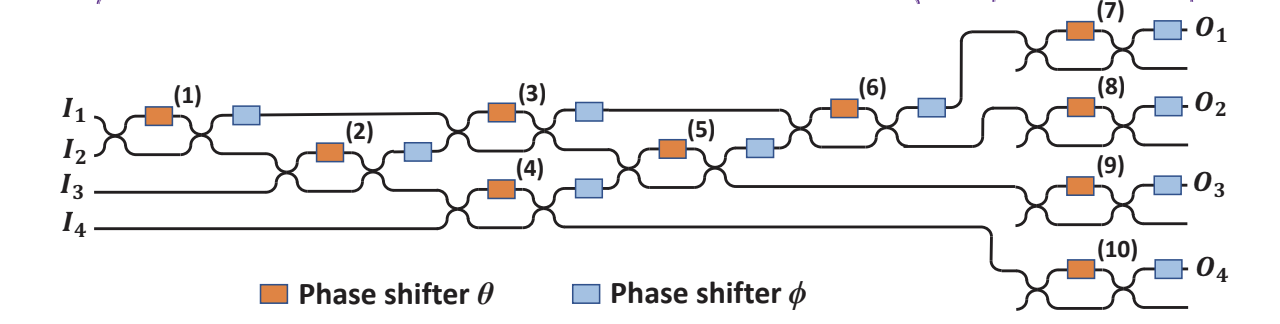
\includegraphics[scale=0.7]{images/cascadedMZI.png}
	\caption{Schematic diagram of a 4x4 MZI based photonic neuron \cite{8961101}}
	\label{4x4mzi}
\end{figure}

As is evident from the picture, the hardware complexity grows exponentially as the number of parameters increase, which is not really practical as the number of parameters in a neural network is usually very large, even reaching billions at times \cite{chowdhery2022palm}. This makes the implementation of such a system very difficult.
 
Another approach to making neural networks in photonics domain is using MicroRing Resonators (MRRs). This uses multiple MRRs in a cascaded fashion to implement a complete spiking neural network \cite{photonics9020120}. Although cascading MRR is somewhat better than cascading MZIs, it still suffers from the same problem of exponential growth of hardware complexity.

\begin{figure}
	\centering
	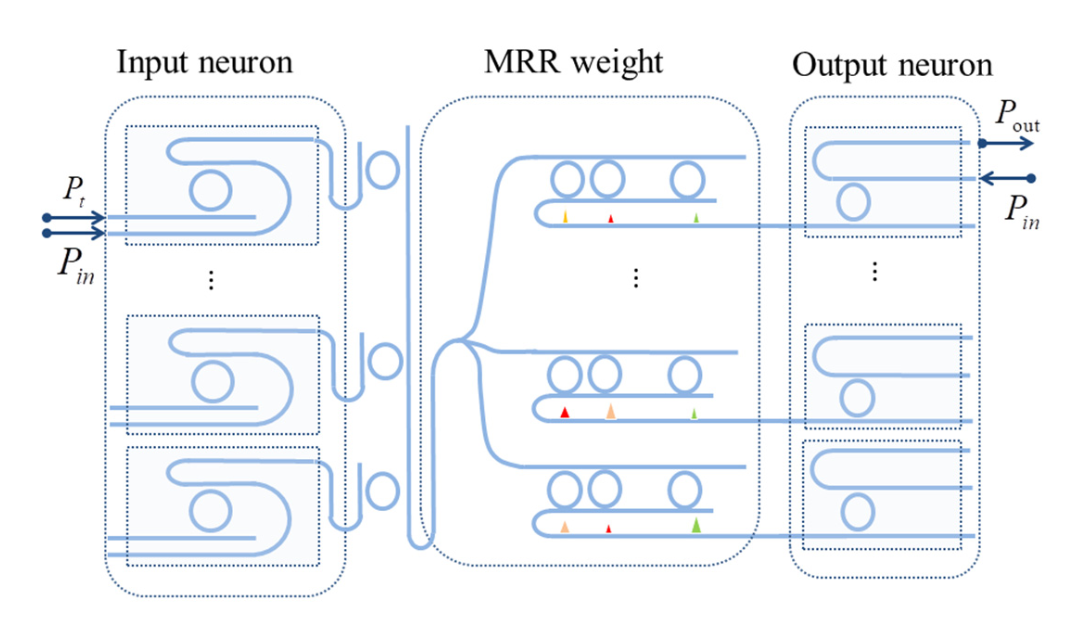
\includegraphics[scale=0.7]{images/cascadedMRR.png}
	\caption{Schematic diagram of a all MRR photonic neuron \cite{photonics9020120}}
\end{figure}

One way to overcome this issue is to use one resuable component for the repetitive operations of the neural network. Just like how GPU were employed for neural net calculations because they were efficient at parallel and repeptetive operations, we can use a small reusable neuron and reuse for the entire neural network.

Following in this path, the structure known as PEMAN \cite{demarinisCodesignedIntegratedPhotonic2022} was introduced. PEMAN stands for Photonic Electronic Multipication Accumulation Neuron. It proposes a hybrid photonic electronic neuron that can be reused many times to implement a complete neural network. The structure of PEMAN is shown in figure \ref{peman}.

\begin{figure}
	\centering
	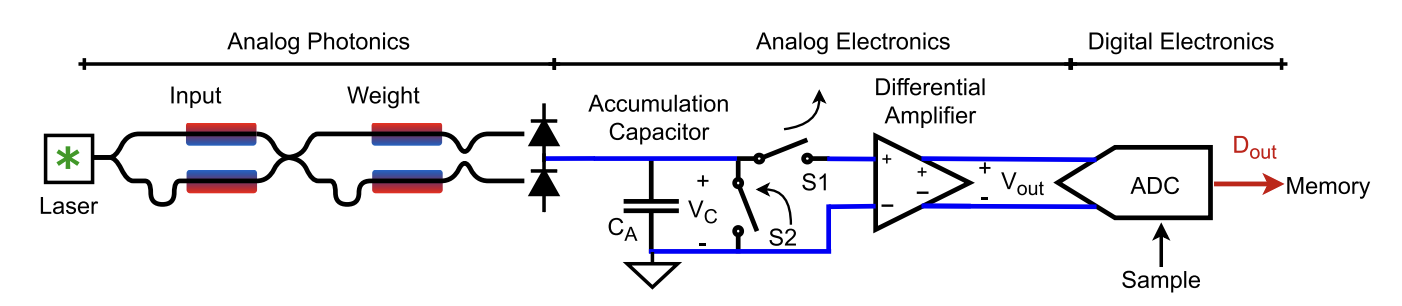
\includegraphics[width=\textwidth]{images/peman.png}
	\caption{Schematic diagram of a PEMAN \cite{demarinisCodesignedIntegratedPhotonic2022}}
	\label{peman}
\end{figure}

\section{Motivation}

The motivation behind this thesis is to explore the possibility of using a PEMAN like structure to implement a complete neural network. The PEMAN structure is a very good candidate for the implementation of a neural network in the photonic domain. It is highly reusable and can be used to implement a complete neural network. The PEMAN structure is also highly power efficient and can be used to implement a neural network that is highly power efficient.

Conventional methods of using neuromorphic hardware includes training the model on high power hardware like GPUs and then deploying the model on the hardware itself after applying relevant quantization and optimizations. Using GPUs take a lot of power and training and deploying on two different infrastructure is a big privacy leak for many applications. This thesis aims to propose a new learning method to train on the hardware directly to overcome aforementioned issues.

In particular, this thesis aims to explore the creation of a artifical neural network and convolutional neural network architecture using an already proposed architecture, the PEMAN structure. In particular, the feasibility of using PEMAN with a CNN context is explored. It also tries to explore the process of training on the said hardware implementation and study the accuracy and time efficiency of the system.
